\documentclass[border=1 cm]{standalone}

\usepackage{tikz}
\usetikzlibrary{patterns}

\begin{document}

    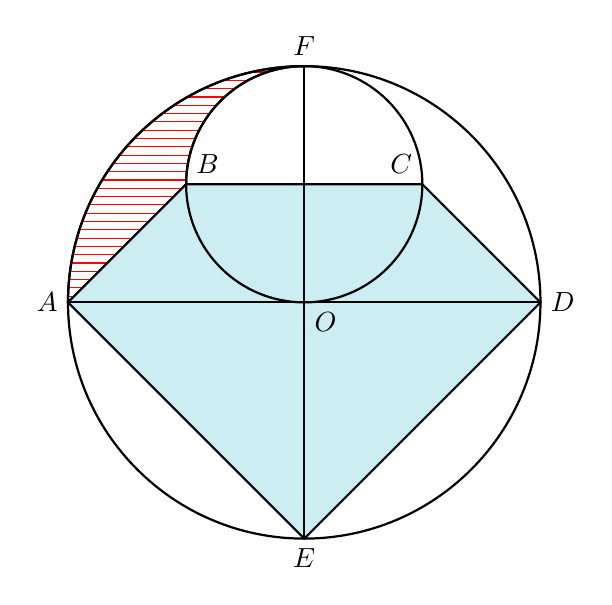
\begin{tikzpicture}[scale=1.5, thick]
        \coordinate (O) at (0,0);
        \coordinate[label=left:$A$] (A) at (-2,0);
        \coordinate[label=right:$D$] (D) at (2,0);
        \coordinate[label=below:$E$] (E) at (0,-2);
        \coordinate[label=above:$F$] (F) at (0,2);
        \coordinate[label=above right:$B$] (B) at (-1,1);
        \coordinate[label=above left:$C$] (C) at (1,1);
        \coordinate (M) at (0,1);
        
        \filldraw[pattern={horizontal lines}, pattern color=red] (A)--(B) arc [start angle=180, end angle=90, radius=1] arc [start angle=90, end angle=180, radius=2] -- cycle;
        \draw (O) circle [radius=2];
        \draw[fill=cyan!80!green!20] (A)--(E)--(D)--(C)--(B)--cycle;
        \draw (M) circle [radius=1];
        \draw (A)--(D) (F)--(E);
        \node at (O) [below right]{$O$};
    \end{tikzpicture}
    
\end{document}